\subsection{Hydrogeologic Radionuclide Transport}
\begin{frame}
  \frametitle{Hydrologic Contaminant Transport}
  \footnotesize{
  In a saturated, reducing environment, contaminants are transported by 
  \textbf{dispersion} and \textbf{advection},  
    \begin{align}
      J &= J_{dis} + J_{adv}\nonumber\\
      &= -n(D_{mdis} + \tau D_m)\nabla C + nvC\nonumber\\ 
      &= -nD\nabla C + nvC \nonumber\\ 
      \intertext{which is, for uniform flow}
      &=\left(-nD_{xx} \frac{\partial C}{\partial x}
             + nv_xC \right)\hat{\imath}
             + \left( -nD_{yy} \frac{\partial C}{\partial y}
            \right)\hat{\jmath}
            + \left( -nD_{zz} \frac{\partial C}{\partial z}
            \right)\hat{k},
      \intertext{where}
      J_{dif} &= \mbox{ Total Dispersive Mass Flux }[kg/m^2/s]\nonumber\\
      J_{adv} &= \mbox{ Advective Mass Flux }[kg/m^2/s]\nonumber\\
      \tau &= \mbox{ Toruosity }[-] \nonumber\\
      n &= \mbox{ Porosity }[\%] \nonumber\\
      D_m &= \mbox{ Molecular diffusion coefficient }[m^2/s]\nonumber\\
      D_{mdis} &= \mbox{ Coefficient of mechanical dispersivity}[m^2/s]\nonumber\\
      D &= \mbox{ Effective Dispersion Coefficient }[m^2/s]\nonumber\\
      C &= \mbox{ Concentration }[kg/m^3],\nonumber\\
    \end{align}
    }

\end{frame}

\begin{frame}
  \frametitle{Hydrologic Contaminant Transport}
  \footnotesize{
  In addition to engineered barriers, their movement is constrained by 
  the solubility limit, 
    \begin{align}
      m_i &\leq V_w C_{sol,i},
    \intertext{and sorption,}
      S &=\frac{V_w(C_0 -C)}{m_s}
    \intertext{where}
      m_i &= \mbox{ mass of isotope i in volume }V_w [kg]\nonumber\\ 
      V_w &= \mbox{ volume of the solution }[m^3]\nonumber\\
      C_{sol,i} &= \mbox{ solubility limit, the maximum concentration of i }[kg_m^3]\nonumber\\
      S &= \mbox{ mass sorbed on the surface }[kg/kg]\nonumber\\
      C_0 &= \mbox{ initial concentration in the solution }[kg_m^3]\nonumber\\
      C &= \mbox{ equilibrium concentration in the solution }[kg/m^3]\nonumber\\
      m_s &= \mbox{ sediment mass }[kg].\nonumber
    \end{align}
    The function $S(C)$ is called a sorption isotherm. 
    }
\end{frame}

\begin{frame}
  \frametitle{Component Interfaces}
  \footnotesize{
  For uniform flow, the governing equation is,

  \begin{align}
    D_x \frac{\partial^2 C}{\partial x^2} +
    D_y \frac{\partial^2 C}{\partial y^2} +
    D_z \frac{\partial^2 C}{\partial z^2} +
    v_x \frac{\partial C}{\partial x}  = R_f \frac{\partial C}{\partial t}.  
    \label{unidirflow}
  \end{align}

  \begin{figure}[htp!]
    \begin{center}
      \def\svgwidth{\textwidth}
      \input{cyder/images/flow.eps_tex}
    \end{center}
    \caption{The boundaries between components are robust interfaces defined by 
    Source Term, Dirichlet, Neumann, and Cauchy boundary conditions.}
    \label{fig:flow}
  \end{figure}
  }
\end{frame}

\begin{frame}
  \frametitle{Boundary Conditions}
  \footnotesize{
    \textbf{First, specified-head or Dirichlet type} boundary conditions define a specified species 
    concentration
    
    \begin{align}
      C(\vec{r},t) = C_0(\vec{r},t)\hspace{1mm}\mbox{ for } \left( \vec{r} \right) \in 
      \Gamma.
    \end{align}
    
    \textbf{Second, specified-flow, or Neumann type} boundary conditions describe a full set of 
    concentration gradients 
    
    \begin{align}
      \frac{\partial C(\vec{r},t)}{\partial r} &= nD\vec{J}(t) \hspace{1mm}\mbox{ for } 
      \vec{r} \in \Gamma.
      \intertext{where}
      \vec{r} &= \mbox{ position vector }\nonumber\\
      \Gamma &= \mbox{ domain boundary }\nonumber\\
      \vec{J}(t) &= \mbox{ solute mass flux } [kg/m^2\cdot s].\nonumber
    \end{align}
    
    \textbf{Third, head-dependent, or Cauchy type}, defines a solute 
    flux along the boundary,
    
    \begin{align}
      -D\frac{\partial C}{\partial x} + v_xC &= v_xC(\vec{r},t).
      \intertext{where}
      D &= \mbox{ hydrodynamic dispersion coefficient } [m^2/s]\nonumber\\
      v_x &= \mbox{ outward fluid flux} [m/s]\nonumber\\
    \end{align}  
  }
\end{frame}

\begin{frame}
  \frametitle{Radionuclide Transport: Mixed Cell}
  % Waste Form
  \begin{figure}[h!]
    \begin{center}
      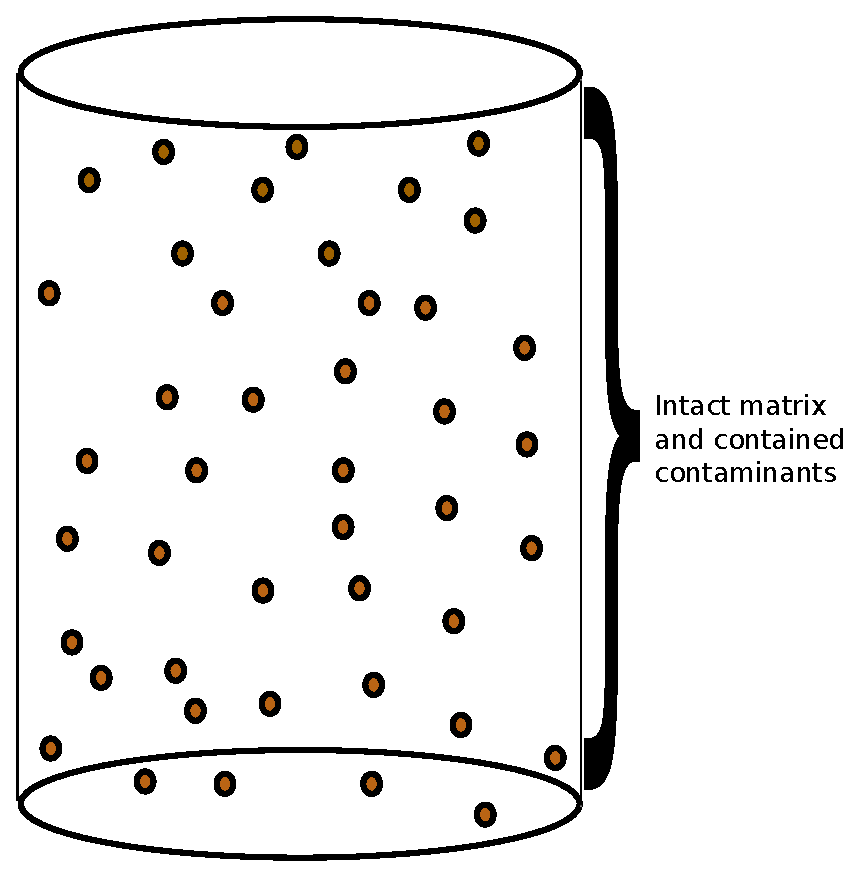
\includegraphics[height=.6\textwidth]{cyder/images/mixed_cell_whole.eps}
    \end{center}
  \end{figure}
\end{frame}

\begin{frame}[ctb!]
  \frametitle{Radionuclide Transport: Mixed Cell}
  % Waste Form
  \begin{figure}[h!]
    \begin{center}
      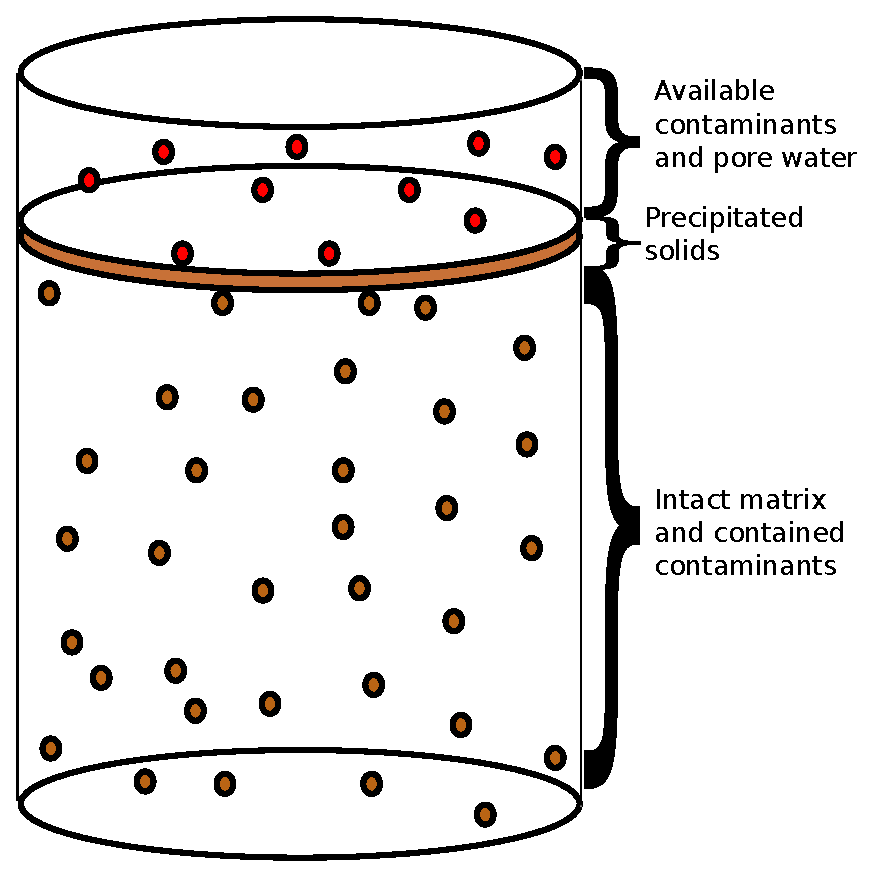
\includegraphics[height=.6\textwidth]{cyder/images/mixed_cell_degraded.eps}
    \end{center}
  \end{figure}
\end{frame}

\begin{frame}
  \frametitle{Radionuclide Transport: Rate Based Congruent Release}
  \footnotesize{
  Contaminants are released congruently with degradation of the component.

  That is, for a rate of $\epsilon [\%]$ per year, where the initial condition is some 
  contained mass, $m_0$, the boundary conditions supplied to external components 
  at the outer boundary $r_{bc}$are :

  \begin{align}
    \intertext{Source Term}
    \dot{m} &= \epsilon m_0
    \intertext{Dirichlet}
    C(r_{bc}) &= \dot{m}/V_w 
    \intertext{Neumann}
    \frac{\partial C}{\partial r} &= ( \dot{m}/V_w - C_{ext} )/(r_{ext} - r_{in})
    \intertext{Cauchy}
    -D \frac{\partial C}{\partial x}\big|_{x=x_{bc}} + v_xc &= vC(x_{bc}) 
  \end{align}
  }
\end{frame}

\begin{frame}
  \frametitle{Radionuclide Transport: Lumped Parameter Transport Model}

\begin{figure}[htbp!]
  \begin{center}
    \def\svgwidth{\textwidth}
    \input{cyder/images/lumpedseries.eps_tex}
  \end{center}
  \caption{ For systems in which the flow can be assumed constant, it is 
  possible to model a system of volumes as a connected lumped paramter models 
  according to a relationship between the incoming concentration, $C_{in}(t)$, 
  and the outgoing concentration, $C_{out}(t)$.}
  \label{fig:lumpedseries}
\end{figure}
\footnotesize{
  \begin{align}
  C_{out}(t) &= \int_0^\infty C_{in}(t-t')g(t')e^{-\lambda t'}dt'
  \label{lumped2}
  \intertext{where}
  t'  &= \mbox{ time of entry }[s]\nonumber\\
  t-t'  &= \mbox{ transit time }[s]\nonumber\\
  g(t-t')  &= \mbox{ response function, a.k.a. transit time 
  distribution}[-]\nonumber]\\
  \lambda &= \mbox{ radioactive decay constant, 1 to neglect}[s^{-1}]
\end{align}
}
\end{frame}


\begin{frame}
  \frametitle{Radionuclide Transport: Lumped Parameter Transport Model}
\footnotesize{
Selection of the response function is usually based on experimental tracer 
results. Canonical forms include :
\begin{align}
  \mbox{the Piston Flow Model (PFM), } g(t') &= \delta{(t'-t_t))}\\
  \mbox{ the Exponential Model (EM), } g(t') &= 
  \frac{1}{t_t}e^{-\frac{t'}{t_t}}\\
  \mbox{ and the Dispersion Model (DM), } g(t') &= \frac{\left[ \left( \frac{t\pi t'}{t_t Pe} \right) 
  (\frac{1}{t'})e^{- \left( 1- \frac{t'}{t_t}  \right)^2} 
  \right]}{\frac{4t'}{t_tPe}}, 
  \intertext{where}
  Pe  &= \mbox{ Peclet number }[-]\nonumber\\
  t_t  &= \mbox{ mean tracer age }[s]\nonumber\\
    &= t_w \mbox{ if there are no stagnant areas}\nonumber\\
  t_w  &= \mbox{ mean residence time of water}[s].\nonumber\\
\intertext{The solutions to these for constant concentration at the source 
boundary give}
  C(t) &=\begin{cases}
    PFM & C_0e^{-\lambda t_t}\\
    EM  & \frac{C_0}{1+\lambda t_t}\\
    DM  & \frac{C_0e^{Pe\sqrt{\left( 1-(1+\frac{4\lambda t_t}{Pe})\right)}}}{2}\\
  \end{cases}
  \label{lumpedsolns}
\end{align}
}
\end{frame}

\begin{frame}
  \frametitle{Radionuclide Transport: 1D Semi-Infinite, Cauchy B.C.}
  \footnotesize{
\begin{figure}[htbp!]
  \begin{center}
    \def\svgwidth{.5\textwidth}
    \input{cyder/images/1dinf.eps_tex}
  \end{center}
  \caption{A one dimensional, semi-infinite model, unidirectional flow,
  solution with Cauchy and Neumann B.C.s}
  \label{fig:1dinf}
\end{figure}
The solution is given (Leij and van Genuchten, \cite{leij_analytical_1991})  as :
\begin{align}
  C(x,t) = \frac{C_0}{2}\Bigg[&\erfc{\frac{L-v_xt}{2\sqrt{D_Lt}}} 
  + \frac{1}{2} \left(\frac{v_x^2t}{\pi D_L}\right)^{1/2}e^{\frac{-( L - 
  v_xt)^2}{4D_Lt}}\nonumber\\
  &- \frac{1}{2}\left( 
  1+\frac{v_xL}{D_L}+\frac{v_x^2t}{D_L}\right)e^\frac{v_xL}{D_L}\erfc{\left[\frac{L-V_xt}{2\sqrt{D_Lt}}\right]} 
  \Bigg]
  \end{align}
  }
\end{frame}

